%(BEGIN_QUESTION)
% Copyright 2006, Tony R. Kuphaldt, released under the Creative Commons Attribution License (v 1.0)
% This means you may do almost anything with this work of mine, so long as you give me proper credit

Følgende differansetrykksensor bruker et matchet par med tøyningsmålere. Når differansetrykket øker, blir den ene tøyningsmåleren komprimert mens den andre strekkes. Et voltmeter registrerer ubalansen i brokretsen og viser denne som en trykkmåling. Polaritetssymbolene ved voltmeteret i diagrammet viser hvilken polaritet som kreves for å drive instrumentet oppover på skalaen:

$$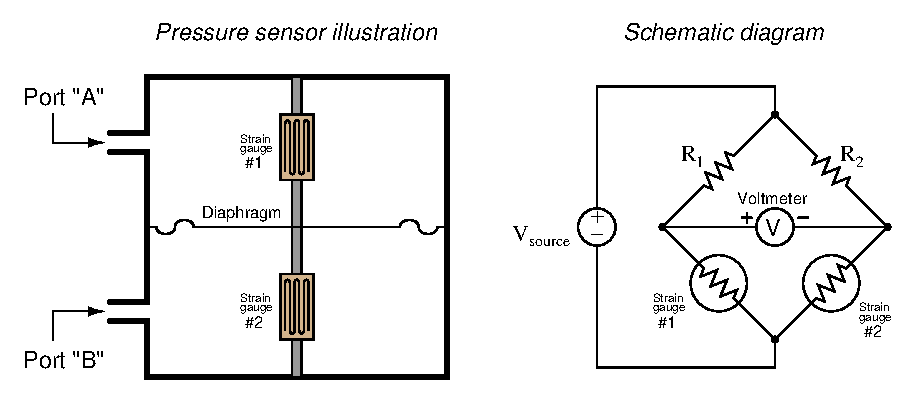
\includegraphics[width=15.5cm]{i00468x01.eps}$$

\begin{itemize}
\item{} Identifiser hvilken port som er «høytrykksporten»
\item{} Identifiser hva voltmeteret vil vise hvis fast motstand $R_1$ får brudd
\item{} Identifiser en komponentfeil som vil drive voltmeteret fullt opp på skalaen («peg» positiv)
\item{} Identifiser en annen komponentfeil som vil drive voltmeteret fullt opp på skalaen («peg» positiv)
\end{itemize}

\vfil

\underbar{file i00468}
\eject
%(END_QUESTION)





%(BEGIN_ANSWER)

Dette er en vurderingsoppgave. Ingen svar eller hint oppgis!

%(END_ANSWER)





%(BEGIN_NOTES)

\begin{itemize}
\item{} Hvilken port er «høytrykksporten»: {\bf Port «A»}
\item{} Hva skjer hvis fast motstand $R_1$ får brudd: {\bf Voltmeteret går helt ned på skalaen («peg» negativ)}
\item{} Identifiser en komponentfeil som vil drive voltmeteret fullt opp på skalaen («peg» positiv):
\item\item{} {\bf (1) Tøyningsmåler \#1 får brudd}
\item\item{} {\bf (2) Tøyningsmåler \#2 blir kortsluttet}
\item\item{} {\bf (3) $R_1$ blir kortsluttet}
\item\item{} {\bf (4) $R_2$ får brudd}
\end{itemize}

\vskip 10pt

For å avgjøre hvilken side som er «høytrykksport», må vi først finne hvilken tøyningsmåler som gir positiv signalendring ved strekk. Fra brokoblingen ser vi at tøyningsmåler \#1 må øke i motstand for å gi positiv voltmeteravlesning. Dermed må port «A» være høytrykksporten, fordi et påført trykk der vil sette tøyningsmåler \#1 i strekk (og samtidig komprimere tøyningsmåler \#2, som også bidrar til positiv voltmeterindikasjon).

\vskip 10pt

Enhver komponent som feiler slik at venstre terminal på voltmeteret blir mer positiv, eller høyre terminal blir mer negativ, vil gi en større positiv voltmeterverdi.

%(END_NOTES)
